\documentclass[11pt]{beamer}
% \usetheme{Boadilla}
  \usetheme{default}


% acronyms for text or math mode
\newcommand {\ccast} {\mbox{\small CCAST}}
\newcommand {\cris} {\mbox{\small CrIS}}

\newcommand {\airs} {\mbox{\small AIRS}}
\newcommand {\iasi} {\mbox{\small IASI}}
\newcommand {\idps} {\mbox{\small IDPS}}
\newcommand {\nasa} {\mbox{\small NASA}}
\newcommand {\noaa} {\mbox{\small NOAA}}
\newcommand {\nstar} {\mbox{\small STAR}}
\newcommand {\umbc} {\mbox{\small UMBC}}
\newcommand {\uw}   {\mbox{\small UW}}

\newcommand {\fft}  {\mbox{\small FFT}}
\newcommand {\ifft} {\mbox{\small IFFT}}
\newcommand {\fir}  {\mbox{\small FIR}}
\newcommand {\fov}  {\mbox{\small FOV}}
\newcommand {\for}  {\mbox{\small FOR}}
\newcommand {\ict}  {\mbox{\small ICT}}
\newcommand {\ils}  {\mbox{\small ILS}}
\newcommand {\igm}  {\mbox{\small IGM}}
\newcommand {\opd}  {\mbox{\small OPD}}
\newcommand {\rms}  {\mbox{\small RMS}}
\newcommand {\zpd}  {\mbox{\small ZPD}}
\newcommand {\ppm}  {\mbox{\small PPM}}
\newcommand {\srf}  {\mbox{\small SRF}}
\newcommand {\sdr}  {\mbox{\small SDR}}

\newcommand {\ES} {\mbox{\small ES}}
\newcommand {\SP} {\mbox{\small SP}}
\newcommand {\IT} {\mbox{\small IT}}
\newcommand {\SA} {\mbox{\small SA}}

\newcommand {\ET} {\mbox{\small ET}}
\newcommand {\FT} {\mbox{\small FT}}

% abbreviations, mainly for math mode
\newcommand {\real} {\mbox{real}}
\newcommand {\imag} {\mbox{imag}}
\newcommand {\atan} {\mbox{atan}}
\newcommand {\obs}  {\mbox{obs}}
\newcommand {\calc} {\mbox{calc}}
\newcommand {\sinc} {\mbox{sinc}}
\newcommand {\psinc} {\mbox{psinc}}
\newcommand {\std} {\mbox{std}}

% symbols, for math mode only
\newcommand {\wn} {\mbox{cm$^{-1}$}}
\newcommand {\lmax} {L_{\mbox{\tiny max}}}
\newcommand {\vmax} {V_{\mbox{\tiny max}}}

\newcommand {\tauobs} {\tau_{\mbox{\tiny obs}}}
\newcommand {\taucal} {\tau_{\mbox{\tiny calc}}}
\newcommand {\Vdc}  {V_{\mbox{\tiny DC}}}

\newcommand {\rIT} {r_{\mbox{\tiny\textsc{ict}}}}
\newcommand {\rES} {r_{\mbox{\tiny\textsc{es}}}}
\newcommand {\robs} {r_{\mbox{\tiny obs}}}

\newcommand {\rITobs} {r_{\mbox{\tiny\textsc{ict}}}^{\mbox{\tiny obs}}}
\newcommand {\rITcal} {r_{\mbox{\tiny\textsc{ict}}}^{\mbox{\tiny cal}}}

\newcommand {\ITmean} {\langle\mbox{\small IT}\rangle}
\newcommand {\SPmean} {\langle\mbox{\small SP}\rangle}


\title{AIRS to CrIS translation}
\author{H.~E.~Motteler}
\institute{
  UMBC Atmospheric Spectroscopy Lab \\
  Joint Center for Earth Systems Technology \\
}
\date{\today}
\begin{document}

%----------- slide --------------------------------------------------%
\begin{frame}[plain]
\titlepage
\end{frame}
%----------- slide --------------------------------------------------%
\begin{frame}
\frametitle{AIRS to CrIS translation}

\begin{itemize}
  \item let $c$ be a vector of \airs\ channel radiances and $S$ a
    matrix whose rows are {\airs} {\srf}s tabulated at a 0.1~cm$^{-1}$
    grid

  \item then $d = S^{-1}c$ is the deconvolution of $c$ on that grid

  \item this can be reconvolved with a double Fourier transform
    to the \cris\ user grid

  \item the useful channels are the intersection of the AIRS and
    \cris\ bands

  \item the stability of $S^{-1}$ is significantly improved with the
    L1c in comparison with the L1b channel set, and further improved
    with a spacing constraint that drops a few of the closest L1c
    channels

\end{itemize}

\end{frame}
%----------- slide --------------------------------------------------%
\begin{frame}
\frametitle{AIRS to CrIS validation}

\begin{itemize}
  \item ``true CrIS'' -- start with kcarta radiances on a
    0.0025~cm$^{-1}$ grid and convolve to the \cris\ user grid

  \item ``true AIRS'' -- start with kcarta radiances as above and
    convolve (with our tabulated {\srf}s) to \airs\ 1c channels

  \item ``AIRS CrIS'' -- start with true \airs, deconvolve to an
    intermediate 0.1~cm$^{-1}$ grid, and reconvolve to \cris
    
  \item compare \airs\ \cris\ with true \cris

  \item compare alternate interpolations with true \cris.  These
    include simple interpolation and interpolation rather than
    deconvolution to the intermediate grid.  Neither worked as well
    as deconvolution

  \item the following tests were done with our 49 fitting profiles

\end{itemize}

\end{frame}
%----------- slide --------------------------------------------------%
\begin{frame}
\frametitle{LW spectra}

\begin{center}
  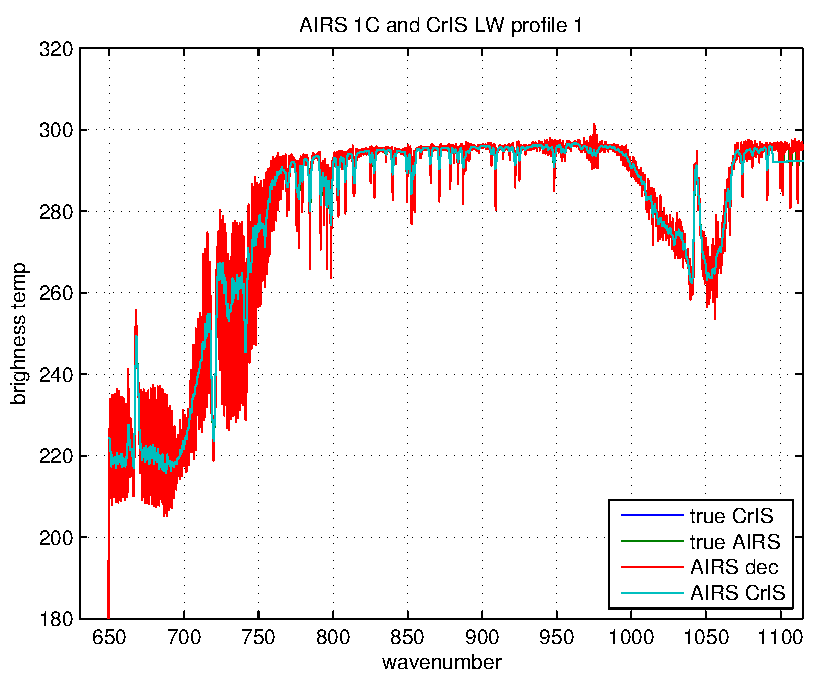
\includegraphics[scale=0.54]{figures/fig_1_LW.pdf}
\end{center}

LW true \cris, true \airs, deconvolved \airs, and \airs\ \cris.  \\
The deconvolved data has significant ringing or overshoot but \\
also some detail not apparent in the original spectra.

\end{frame}
%----------- slide --------------------------------------------------%
\begin{frame}
\frametitle{LW residual}

\begin{center}
  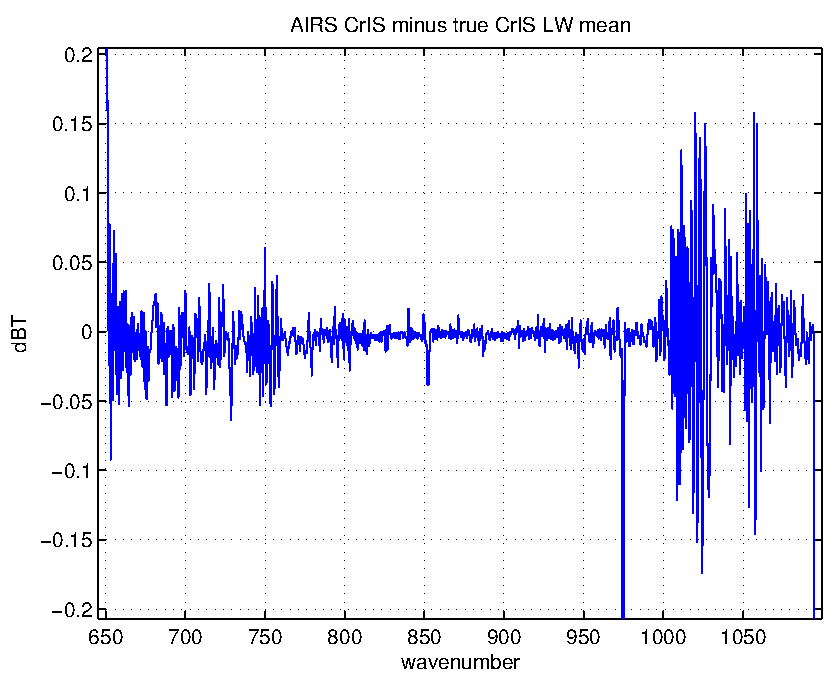
\includegraphics[scale=0.54]{figures/fig_2_LW.pdf}
\end{center}

LW \airs\ \cris\ minus true \cris, the mean of residuals over 49
fitting profiles.

\end{frame}
%----------- slide --------------------------------------------------%
\begin{frame}
\frametitle{MW spectra}

\begin{center}
  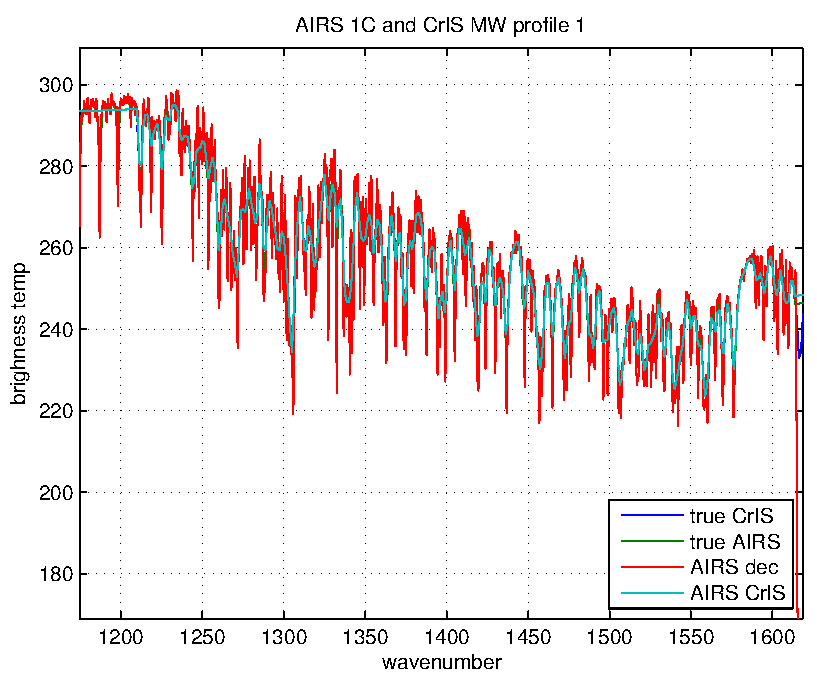
\includegraphics[scale=0.54]{figures/fig_1_MW.pdf}
\end{center}

MW true \cris, true \airs, deconvolved \airs, and \airs\ \cris.  \\
The deconvolved data has significant ringing or overshoot but \\
also some detail not apparent in the original spectra.

\end{frame}
%----------- slide --------------------------------------------------%
\begin{frame}
\frametitle{MW residual}

\begin{center}
  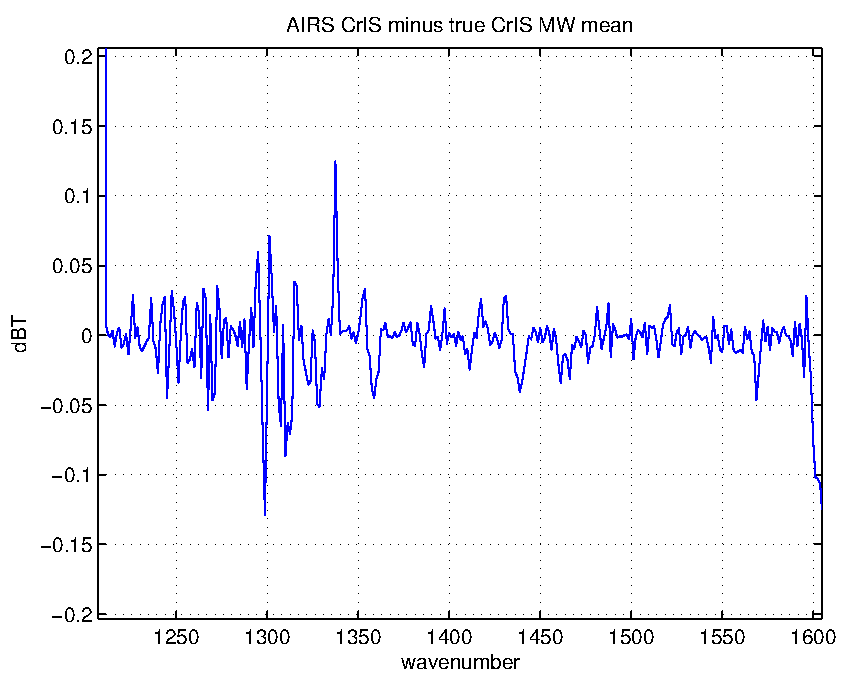
\includegraphics[scale=0.54]{figures/fig_2_MW.pdf}
\end{center}

MW \airs\ \cris\ minus true \cris, the mean of residuals over 49
fitting profiles.

\end{frame}
%----------- slide --------------------------------------------------%
\begin{frame}
\frametitle{SW spectra}

\begin{center}
  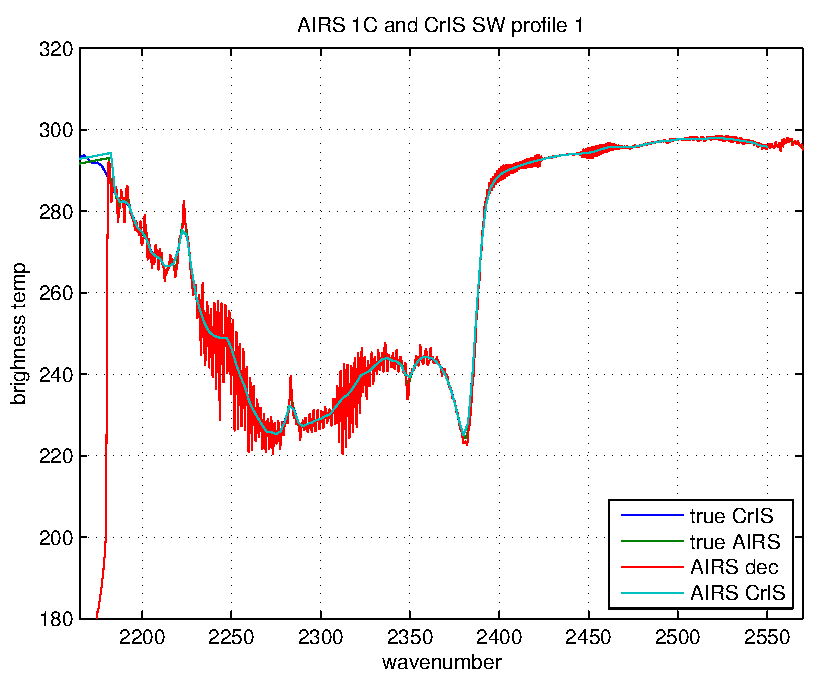
\includegraphics[scale=0.54]{figures/fig_1_SW.pdf}
\end{center}

SW true \cris, true \airs, deconvolved \airs, and \airs\ \cris.  \\
The deconvolved data has significant ringing or overshoot but \\ 
also some detail not apparent in the original spectra.

\end{frame}
%----------- slide --------------------------------------------------%
\begin{frame}
\frametitle{SW residual}

\begin{center}
  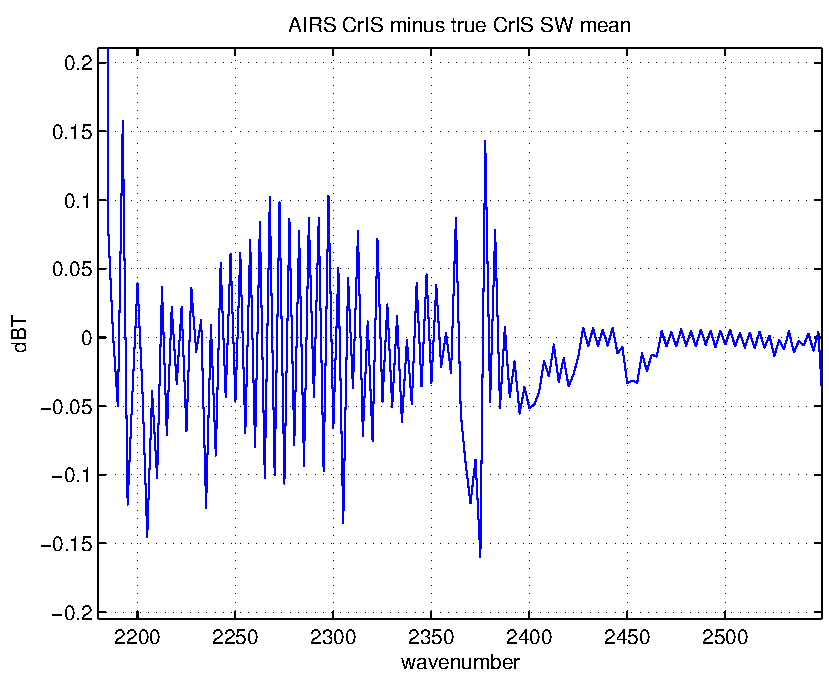
\includegraphics[scale=0.54]{figures/fig_2_SW.pdf}
\end{center}

SW \airs\ \cris\ minus true \cris, the mean of residuals over 49
fitting profiles.

\end{frame}
%----------- slide --------------------------------------------------%

\end{document}

